\section{Dekodierung der Farben}

Das 1-pixel breite Bild wird im HSV-Raum gefiltert (einfaches Thresholding) um
die Blaue Farbe zu entfernen. Zum Teil bleiben  an  den  R\"andern  der  Ringe
kleine Fragmente \"ubrig,  welche  mit  Hilfe einer Dillation entfernt werden.
Das Resultat ist in der Abbildung \ref{fig:9} zu sehen.

\begin{figure}[H]
    \centering
    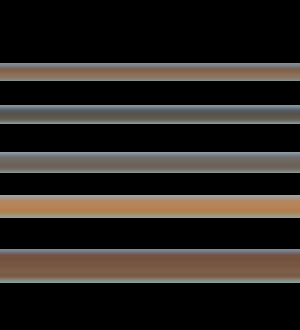
\includegraphics[width=.4\linewidth]{images/9}
    \caption{Farbringe mit Thresholding isoliert.}
    \label{fig:9}
\end{figure}

Das Bild wird aufgeteilt in mehrere Bilder (in diesem  Fall  5, ein Bild f\"ur
jeder Ring), und der Mittelwert  der Pixel wird berechnet um eine Endg\"ultige
Farbe zu erlangen.

Die Weiss, Grau, Silber, und Schwarze  Farben  werden  im  RGB-Farbraum zuerst
detektiert,  indem die RGB-Kan\"ale miteinander verglichen  werden.  Wenn  sie
etwa  den  gleichen  Wert  aufweisen, wird weiter mit  Thresholding  der  Wert
bestummen.

Haben die Kan\"ale andere Werte, so  kann  angenommen  werden, dass es sich um
eine  Farbe  handelt.  Die MATLAB-Funktion \textit{rgb2ind} wird verwendet, um
eine  Korrelation  zwischen  die sieben \"ubrigbleibenden  Farben  zu  finden.

Zu  guter   Letzt  werden  die  Werte  nach  einer  Tabelle\cite{ref:resistorcodes}  (siehe  Abbildung
\ref{fig:resistorchart}) dekodiert. Momentan erfolgt dies in beide Richtungen,
weil bei vielen Widerst\"anden die Richtung zweideutig ist.

\begin{figure}[t]
    \centering
    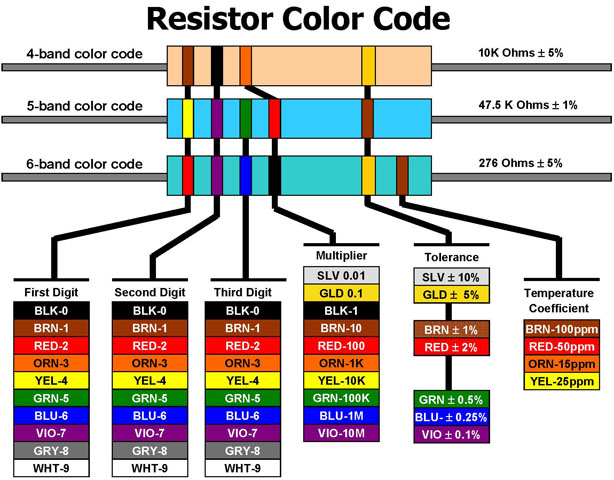
\includegraphics[width=\linewidth]{images/resistorchart}
    \caption{Widerstandswerte\cite{ref:resistorcodes}}
    \label{fig:resistorchart}
\end{figure}

Das Endresultat ist in der Abbildung \ref{fig:10} zu sehen.

\begin{figure}[t]
    \centering
    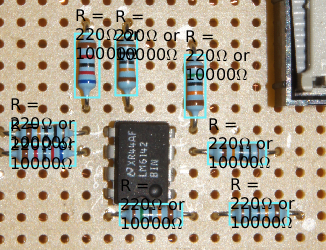
\includegraphics[width=.8\linewidth]{images/10}
    \caption{Endresultat}
    \label{fig:10}
\end{figure}

